\chapter{Lavorazioni per asportazione di truciolo}\label{chp:AsportaTruciolo}
Il principio di funzionamento delle lavorazioni per asportazione di truciolo è
differente da quanto visto fin ora.
Nelle lavorazioni per deformazione plastica si avevano delle deformazioni lente.
\emph{"Per cui il materiale aveva il tempo di adattarsi"}.
Per l'asportazione di truciolo così non può essere. Infatti si suppone che il
materiale venga rotto, tra l'altro il più rigidamente possibile.
Dunque le deformazioni richieste devono essere a più alta velocità.
Ciò però crea delle problematiche non indifferenti:
\begin{itemize}
\item deformazioni veloci non sono rappresentabili tramite prove classiche.
\item Si rende necessario idealizzare il processo e man mano aggiungere ipotesi più realistiche.
\end{itemize}

\section{Introduzione}
Nelle lavorazioni viste fin ora si portava il materiale a deformazione, anche per la tranciatura
nel momento in cui il materiale subiva una deformazione critica fino all'innesco di cricche da cui poi
avveniva la separazione del materiale.
Per l'asportazione del truciolo non può essere così: la deformazione avviene in tempi molto più rapidi,
per cui il materiale ha comportamenti differenti da quelli visti in precedenza.
Inoltre, considerando il materiale di scarto, per le lavorazioni a deformazione si può recuperare ed 
eventualmente riciclare.
Per le lavorazioni ad asportazione la cosa è molto più complicata e difficile.
Il valore del truciolo è pressoché nullo e il suo recupero può essere complicato 
per via delle molteplici varietà di materiale che possono subire tali lavorazioni.
Alla tabella \ref{examp:VantSvant} sono riportati alcuni vantaggi e svantaggi di tali lavorazioni.

\begin{example}{Vantaggi e Svantaggi}
\centering
\begin{tabularx}{\textwidth}{XX}
\toprule
\textbf{Vantaggi} & \textbf{Svantaggi}\\
\midrule
Si possono ottenere tolleranze migliori & Tempo ciclo molto più lento\\
\midrule
Buona finitura superficiale & Scarti di materiale non recuperabili\\
\midrule
\multicolumn{2}{c}{Adatti alla lavorazione di pezzi unici}\\
\midrule
Costo macchina relativamente basso & Spesso è richiesta alta lavorazione manuale\\
\bottomrule
\end{tabularx}
\label{examp:VantSvant}
\end{example}

In industria si sta cercando di eliminare queste lavorazioni per via del tempo ciclo molto elevato.
Sebbene, in abito artigianale stiano avendo un forte sviluppo, sia in termini di automazione,
dunque di tecnologia a bordo macchina; sia di lavorazioni permesse dalle macchine.
Altro grande punto a favore di tali lavorazioni è sicuramente l'adattabilità per 
qualsiasi materiale.

In industria, vengono relegate ad operazioni di finitura del prodotto, dove con una
singola passata si cerca di completare il prodotto e metterlo sul mercato.
Per l'artigianato invece si ha un utilizzo più intensivo, dove con una passata si cerca 
di ottimizzare la quantità di materiale asportato.

Come punto di partenza è utile considerare applicazioni in cui il processo sia completamente
idealizzato.

\section{Taglio ortogonale}
Alla figura \ref{fig:TaglioOrto} sono rappresentati degli esempi di taglio ortogonale.

\begin{figure}
\centering
\subfloat[][\emph{Visualizzazione del taglio ortogonale}\label{fig:TaglioOrto}]
{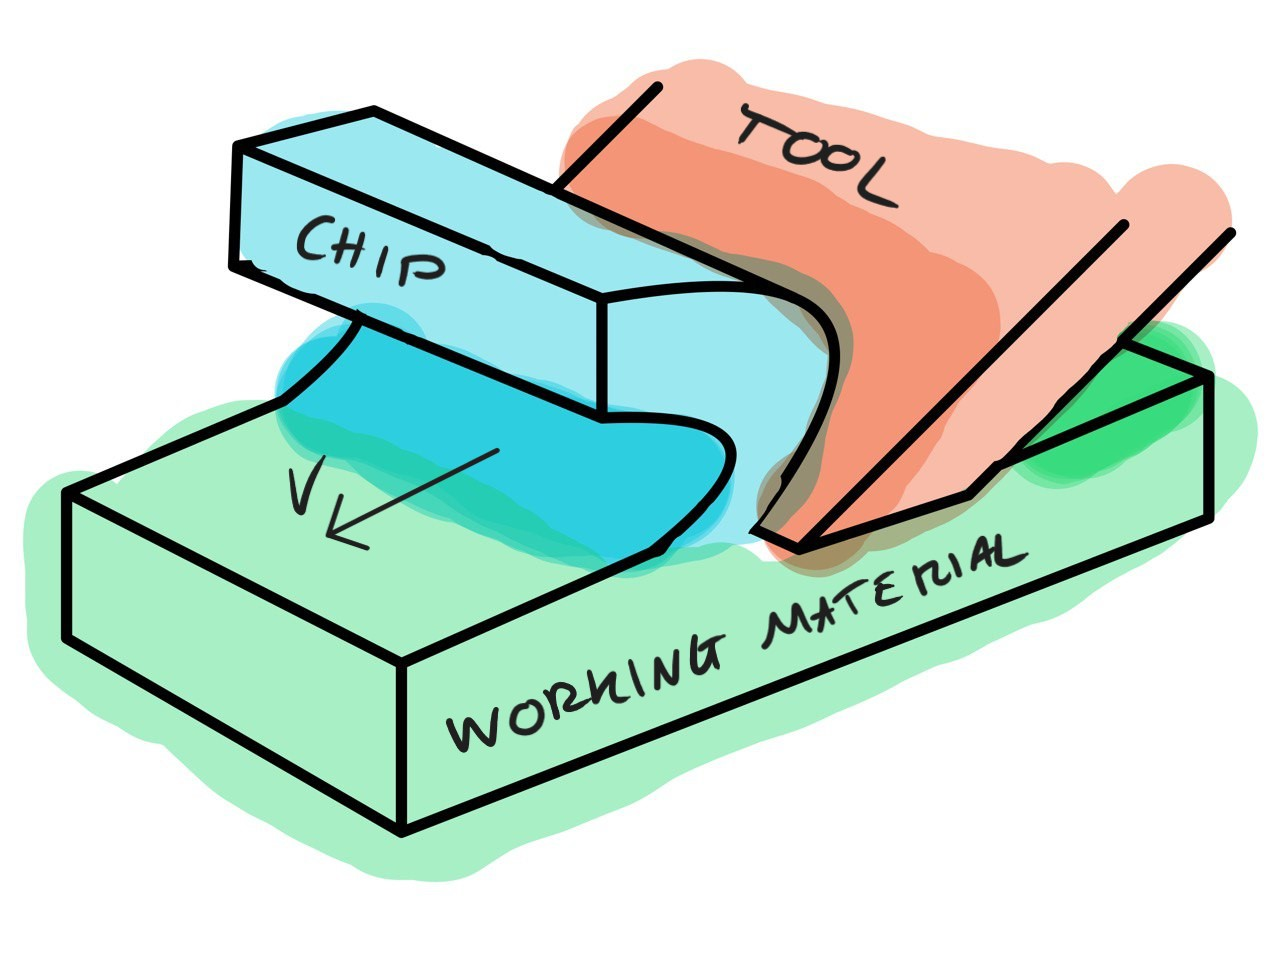
\includegraphics[width = 0.8\textwidth]{TaglioOrto}}\\
\subfloat[][\emph{Parametri del taglio ortogonale}\label{fig:ParamTaglioOrto}]
{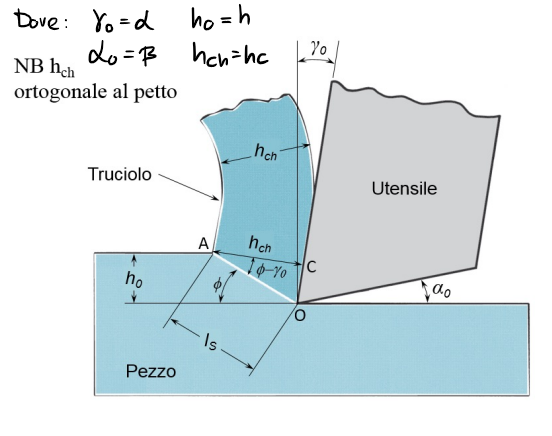
\includegraphics[width=0.7\textwidth]{ParamTaglioOrto}}
\caption{Taglio Ortogonale}\label{fig:TaglioOrto}
\end{figure}
\todo[inline]{Hai fatto una cagata!!! Aggiusta i parametri della figura!!!}
Si dice che il taglio è ortogonale quando la lama dell'utensile è ortogonale alla direzione della velocità di taglio.
Allora si possono definire diversi parametri come riportato nella definizione \ref{def:ParamTaglioOrto}.

\begin{definition}{Parametri del taglio ortogonale}{pramTaglioOrto}
\begin{description}
\item[$\alpha$] Angolo di spoglia superiore o frontale. Da cui
	\begin{description}
	\item[Se $\alpha > 0$] allora si dice che l'utensile ha angolo acuto,
	\item[Se $\alpha < 0$] allora si dice che l'utensile ha angolo ottuso.
	\end{description}
\item[$\theta$] Angolo di spoglia inferiore
\item[$\phi$] Angolo di taglio
\item[$h$] Spessore di taglio indeformato
\item[$h_c$] Spessore del truciolo
\end{description}
\label{def:ParamTaglioOrto}
\end{definition}

Come ipotesi ideale, si considererà che tutta la deformazione del materiale avverrà
solamente sul piano di taglio.
Allora, dai parametri del taglio ortogonale si possono ottenere:
\begin{equation}
r_c = \frac{h}{h_c} = \frac{l_c}{l} := \text{Rapporto di taglio}
\end{equation}
Dove:\\
\begin{tabular}{cl}
$l_c$ & è la lunghezza del truciolo\\
$l$ & è la lunghezza del taglio\\
\end{tabular}
\\
Mentre:
\begin{equation}
F = K \cdot A
\end{equation}
ovvero, la forza necessaria a tagliare il pezzo sarà proporzionale all'area $A$ del piano di taglio 
dovuta dalla lunghezza del piano stesso per la profondità del pezzo in senso ortogonale alla 
figura \ref{fig:ParamTaglioOrto}; in più sarà proporzionale alla pressione $K$ esercitata dall'utensile sul pezzo
Inoltre, si può intuire che: per abbassare l'intensità della forza complessiva per il taglio
sarebbe opportuno aumentare $\phi$, così da limitare l'estensione del piano di taglio e di 
conseguenza la sua area.
Si può ottenere una stima dell'angolo di taglio tramite
\begin{equation}
\tan\phi = \frac{r_c \cos\alpha}{1-r_c\sin\alpha}
\end{equation}
considerando che il rapporto di taglio lo si può misurare abbastanza facilmente dato che:
lo spessore di taglio lo si decide in base alla lavorazione da effettuare, mentre lo
spessore del truciolo lo si può misurare abbastanza facilmente.
Dunque è evidente che l'angolo $\alpha$ lo si vuole molto grande, in modo da generare piani
di taglio molto piccoli: garantendo la necessità di applicare una forza minore.

Risulta utile prestare attenzione alla successiva considerazione.
Il valore di deformazione che si raggiunge con le lavorazioni per asportazione di truciolo
è nettamente più alte che non le deformazioni per lavorazioni tramite deformazione.
Giusto per dare un'idea dell'ordine di grandezza:
\begin{equation}
\dot{\gamma} = \frac{v_s}{d} = \frac{\cos\alpha}{\cos\left(\phi - \alpha\right)} \frac{v}{d} \left[\unit{\s^{-1}}\right]
\end{equation}
nella tecnica, si osservano i seguenti valori:
\begin{description}
\item[Lavorazione per deformazione] $\approx 1 \div 10 \left[\unit{\s^{-1}}\right]$
\item[Lavorazione per asportazione] $\approx 1000 \left[\unit{\s^{-1}}\right]$
\end{description}

\subsection{Fattore di attrito}
Sappiamo che il fattore di attrito ricopre importante ruolo per quanto riguarda questo tipo
di lavorazioni. Ci si deve prestare attenzione.

\begin{equation}
\mu = \frac{\tau_i}{p}
\end{equation}
Di base, questa sarebbe la definizione principale di fattore di attrito.
Se però si osserva il caso del taglio ortogonale, è possibile osservare che secondo
la figura